\chapter{Swiss Terrain 3D}
\label{chap_swiss_terrain_3d}
Kapitel \ref{chap_datengrundlage} behandelte die Datengrundlage für die Terrainvisualisierung. In Kapitel \ref{chap_technologien} wurden Programme und Frameworks zur Erstellung von 3D-Visualisierungen thematisiert. Die technisch notwendigen Grundlagen wurden im Rahmen von Kapitel \ref{chap_render_pipelines} erläutert. Kapitel \ref{chap_algorithmen} befasste sich mit gängigen Datenstrukturen und Algorithmen. Aufbauend auf diesem Vorwissen geht es in diesem Kapitel um die eigentliche Implementierung der Terrainvisualisierung.

\section{Technologie und Anforderungen}
Bevor eine Visualisierung implementiert werden kann, müssen sowohl die Anforderungen als auch die hierfür verwendete Technologie geklärt werden. Eine echtzeitfähige 3D-Visualisierung ist vereinfacht ausgedrückt eine Abfolge von Bildern, welche von der Grafikkarte gezeichnet werden. Diese Bilder werden abhängig vom Blickwinkel der Kamera, den zugrundeliegenden Daten und den Nutzereingaben generiert. Werden die Bilder schnell genug hintereinander gezeichnet, entsteht eine flüssige Animation. Damit eine 3D Visualisierung als Echtzeit bezeichnet werden kann, muss die Visualisierung mit mindestens 30 Bildern pro Sekunde (FPS) gezeichnet werden. Moderne Monitore besitzen jedoch eine wesentlich grössere Spannweite in Bezug auf die Bildwiederholrate. So sind Bildwiederholraten von 60FPS bis hin zu 240FPS keine Seltenheit mehr. Abgesehen von der Bildwiederholrate spielt auch die Auflösung eine wichtige Rolle. Je höher die Auflösung, desto detailgetreuer lässt sich die Visualisierung darstellen. Jedoch braucht es für eine hohe Auflösung in Kombination mit einer hohen Bildwiederholrate auch entsprechend gute Grafikkarten, was wiederum Einfluss auf die erreichbare Zielgruppe hat. Die vorliegende Masterarbeit geht hier deshalb einen Mittelweg und legt folgende Mindestanforderungen an die Visualisierung fest. \textit{Die Visualisierung soll mit mindestens 60 Bildern pro Sekunde und einer Auflösung von 2k (2048px auf 1080px) laufen}.

Nebst den technischen Anforderungen stellt sich auch die Frage auf welchen Plattformen die Anwendung lauffähig sein soll. Der Spielraum ist hier entsprechend gross. Angefangen von nativen Anwendungen welche betriebssystemabhängig sind, bis hin zu Anwendungen auf mobilen Endgeräten sowie komplett betriebssystemunabhängigen Browseranwendungen. Um eine möglichst breite Zielgruppe abzudecken und keinerlei Installationsaufwand aufseiten der Nutzer zu haben, hat sich der Autor für die Implementierung einer webbasierten Anwendung entschieden. 

Wie in Kapitel \ref{chap_technologien} thematisiert, unterstützen moderne Engines wie Unity, Unreal und Godot das Erstellen von browserbasierten Anwendungen. Jedoch ist und bleibt die primäre Zielplattform die nativen Anwendungen. Ausserdem werden bei Engines wie Unity und Unreal entsprechende Lizenzgebühren fällig. Obwohl Engines diverse Programme mitbringen, um das Erstellen von interaktiven Erlebnissen zu vereinfachen, zwingen sie dem Programmierer auch eine vorgegebene Architektur auf. Zudem benötigt insbesondere die Unreal Engine entsprechend gute Hardware, um überhaupt solche Visualisierungen zu entwickeln. Daher hat sich der Autor für webbasierte Frameworks entschieden, bei denen der Browser als primäre Zielplattform gilt und die entsprechende Unterstützung für die modernsten browserbasierten Grafikschnittstellen wie WebGPU anbieten. Da das \acrshort{CAVE}-System der FHGR auf dem Framework ThreeJs basiert und der Autor bereits entsprechende Vorkenntnisse mitbringt, wurde dieses gegenüber BabylonJs präferiert. ThreeJs hat zudem gegenüber BabylonJs den Vorteil, dass auf eine wesentlich grössere Community und ein breites Spektrum von diversen Beispielapplikationen zurückgegriffen werden kann. Zudem ist es mithilfe von Technologien wie Tauri und Electron (siehe Kapitel \ref{chap_technologien}) jederzeit möglich, eine browserbasierte Anwendung nativ auf dem Betriebssystem auszuführen.

\section{Datenvorverarbeitung}
Dem Autor war es wichtig, dass die Datenvorverarbeitung nicht manuell von Hand erfolgen muss. Deswegen wurden alle nachfolgend behandelten Aspekte mithilfe eines Python-Skripts weitestgehend automatisiert und müssen daher nicht manuell getätigt werden. Abbildung \ref{fig_data_preprocessing} zeigt die komplette Datenvorverarbeitung auf einen Blick. Nachfolgend wird auf die einzelnen Teilbereiche genauer eingegangen.
\begin{figure}[H]
    \caption{Übersicht Datenvorverarbeitung (Eigene Darstellung)}
    \includegraphics[width=.8\linewidth]{content/00_assets/cdlod_quadtree.png}
    \label{fig_data_preprocessing}
\end{figure}

\subsection{Herunterladen der Daten}
Sowohl der swissALTI3D als auch der swissIMAGE-Datensatz stehen kostenfrei auf der swisstopo Webseite zum Download bereit (siehe Abbildung \ref{fig_swisstopo_datenbezug}). Zu Beginn wählt der Nutzer den entsprechenden Bereich aus. Dies kann entweder über die Auswahl einer Gemeinde eines Kantons oder über das Definieren eines Bereiches auf der Karte erfolgen (siehe Bereich A in Abbildung \ref{fig_swisstopo_datenbezug}). Anschliessend werden das gewünschte Datenformat sowie die entsprechende Auflösung ausgewählt (siehe Bereich B in Abbildung \ref{fig_swisstopo_datenbezug}). Daraufhin kann eine entsprechende CSV-Datei heruntergeladen werden, welche die Links zu den entsprechenden Datensätzen beinhaltet. Eine Zeile dieser CSV Datei entspricht hierbei jeweils einer km$^2$ Kachel. Damit diese Daten nicht einzeln von Hand manuell heruntergeladen werden müssen, wurde ein Python-Skript geschrieben, welches nur die CSV-Datei benötigt und anschliessend die notwendigen Dateien eigenständig herunterlädt und in die vorkonfigurierten Ordner (definierbar über eine JSON-Datei) ablegt.
\begin{figure}[H]
    \caption{Herunterladen der swisstopo Daten (Eigene Darstellung)}
    \includegraphics[width=.4\linewidth]{content/00_assets/swisstopo_datenauswahl.png}
    \label{fig_swisstopo_datenbezug}
\end{figure}

Die Daten, welche in den CSV-Dateien enthalten sind, erstrecken sich nicht zwingend über einen kontinuierlichen Bereich. Wählt man etwa die Region Sarganserland auf der swisstopo-Webseite aus und setzt anschliessend die km$^2$-Kacheln zu einem Gesamtbild zusammen, wird ersichtlich, dass Lücken vorhanden sind (siehe schwarze Bereiche in der Abbildung \ref{fig_swisstopo_daten_luecken}). Da jedoch die Kacheln auf dem LV95-Koordinatensystem basieren, können die fehlenden Bereiche detektiert, entsprechend in der CSV-Datei hinterlegt und somit die Lücken geschlossen werden (siehe Abbildung \ref{fig_swisstopo_daten_luecken}).

\begin{figure}[H]
    \caption{Lücken in swisstopo-Daten (links) mit automatischer Korrektur (Eigene Darstellung)}
    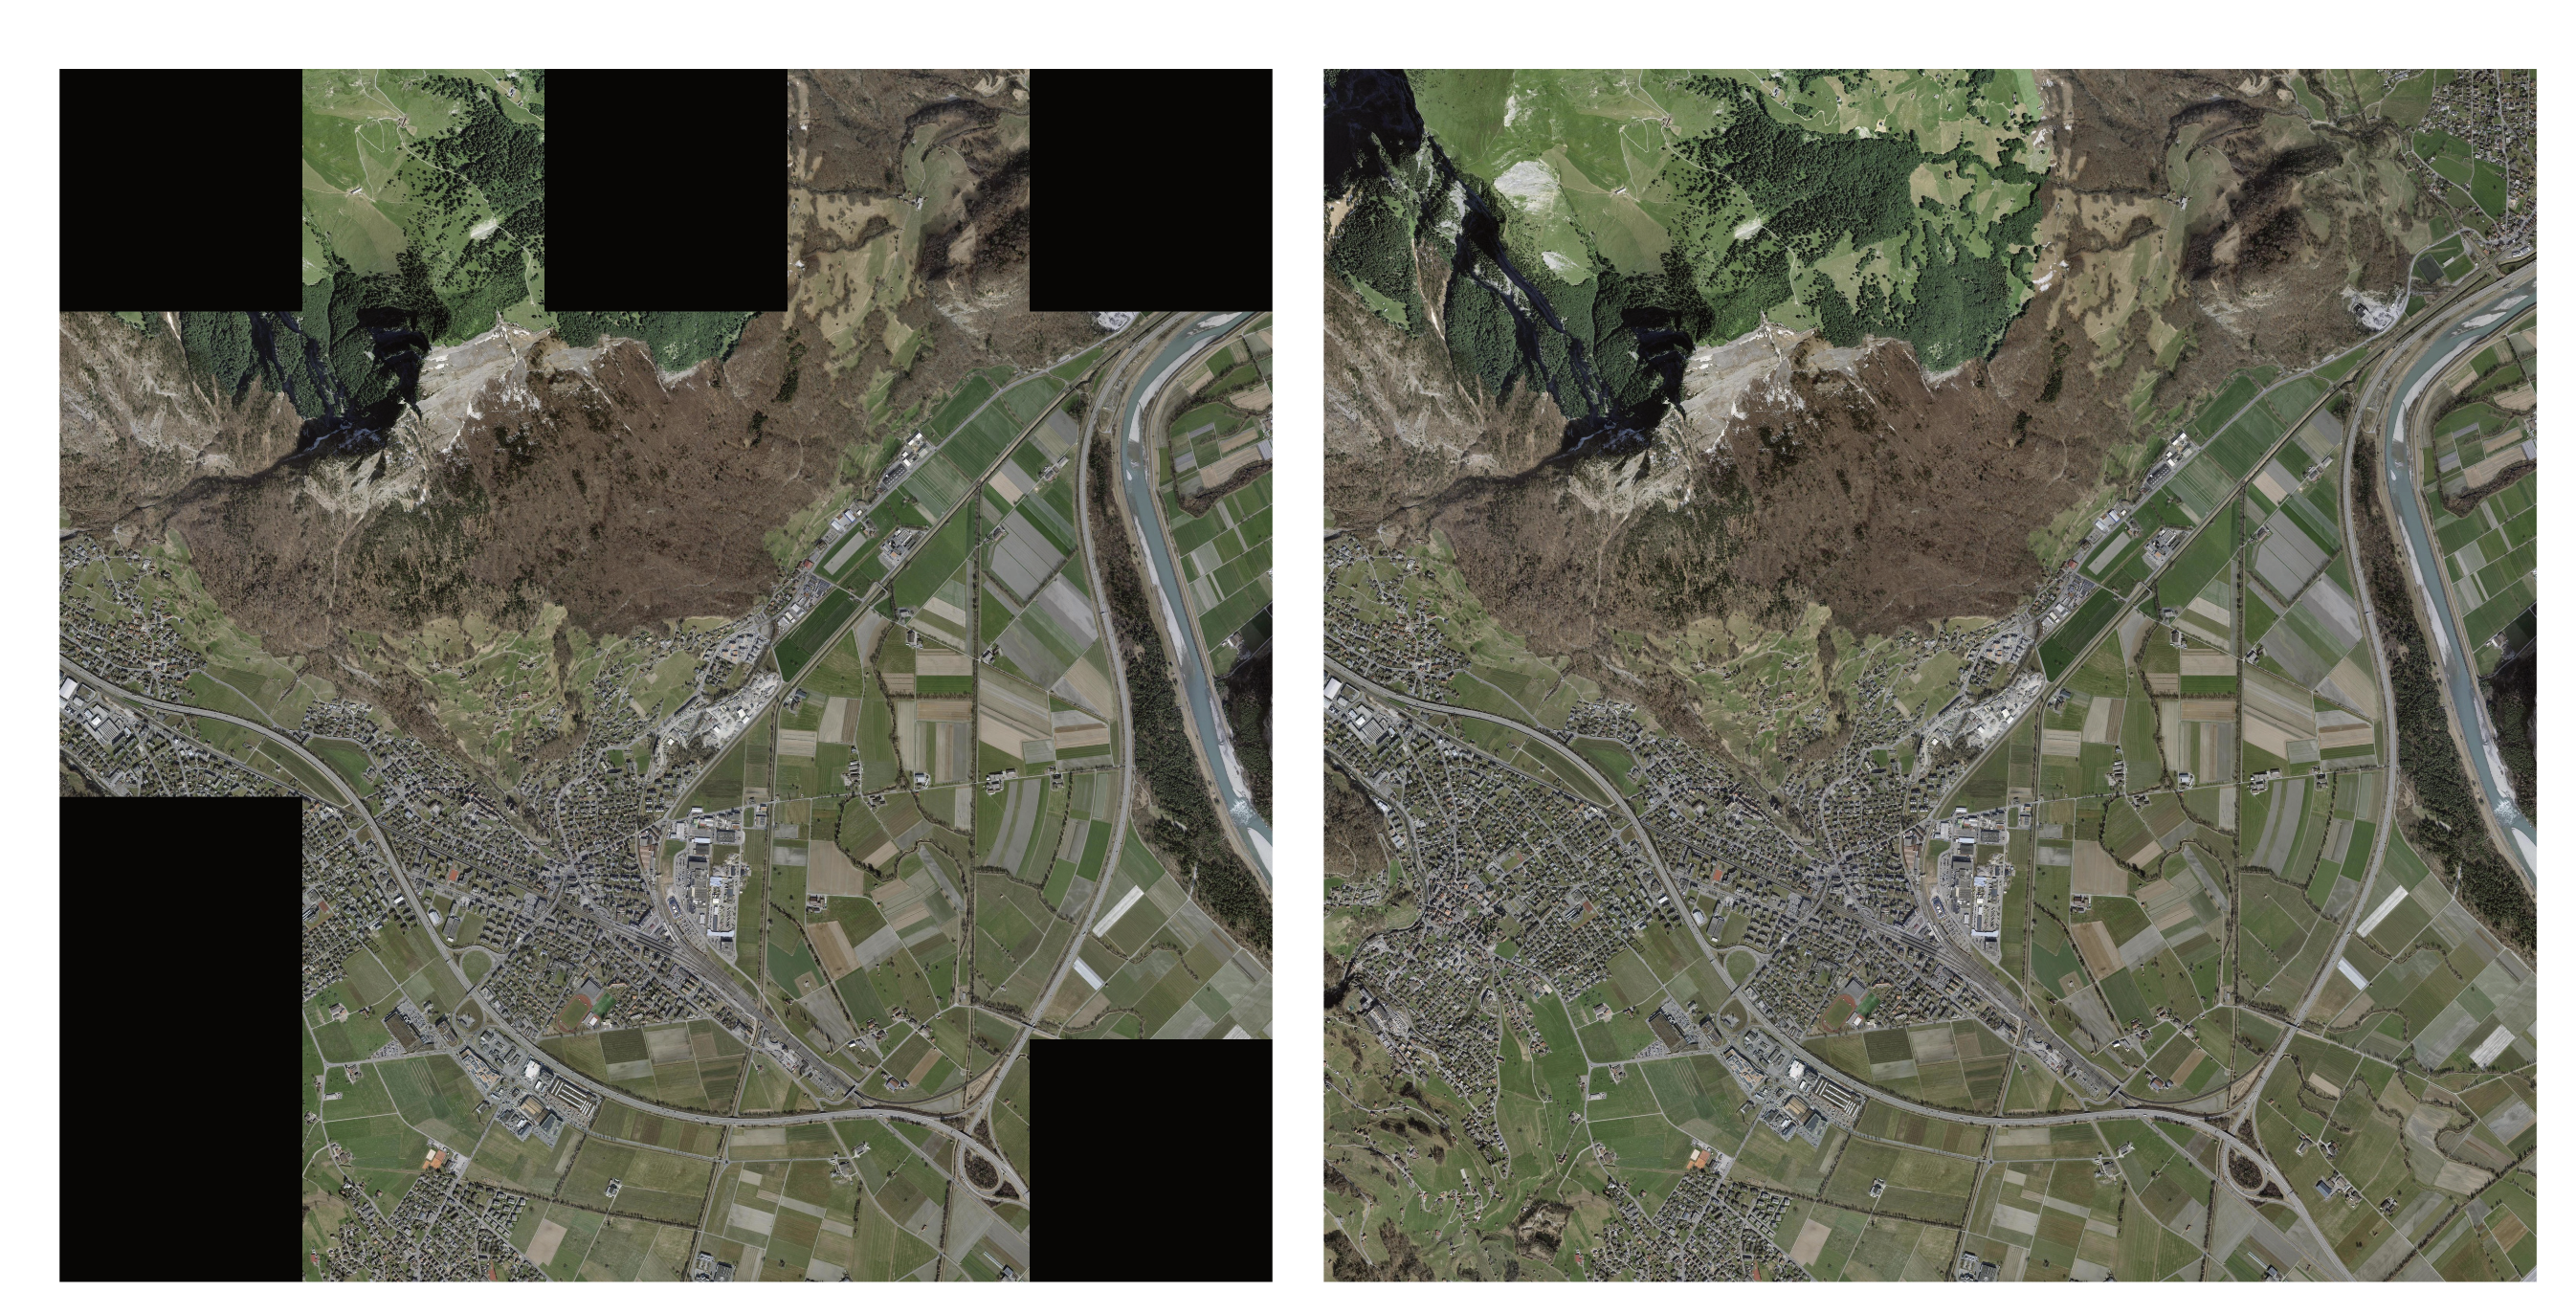
\includegraphics[width=.6\linewidth]{content/00_assets/gesamtbild_mit_luecken.png}
    \label{fig_swisstopo_daten_luecken}
\end{figure}

\subsection{Extrahierung der Höhen- und Bilddaten}
Sind die Daten heruntergeladen, müssen sowohl die Bild- als auch die Höhenwerte aus den GeoTIFF-Dateien extrahiert und als eigenständige Texturen (Bilder) abgespeichert werden. Die Höhenwerte werden hierbei als Graustufenbild gespeichert. Eine weisse Farbe bedeutet hierbei einen hohen, schwarz einen tieferen Wert (siehe Abbildung \ref{fig_heightmap_beispiel}). 
\begin{figure}[H]
    \caption{Extrahierte Höhenwerte als Graustufenbild (Eigene Darstellung)}
    \includegraphics[width=.4\linewidth]{content/00_assets/heightmap_beispiel.png}
    \label{fig_heightmap_beispiel}
\end{figure}

Um die Geopositionsdaten nicht zu verlieren, werden diese in den Dateinamen geschrieben. Da die Daten von swisstopo in Form von km$^2$-Kacheln zur Verfügung gestellt werden, müssen die Kacheln in einem nächsten Schritt zu einem Gesamtbild zusammengesetzt werden. Da die Geoposition jeder Kachel anhand des LV95-Koordinatensystems bekannt ist, können diese anhand der zugehörigen Nord- und Ostachsenwerte zusammengesetzt werden. Hier offenbart sich jedoch das erste Problem mit den Höhenwerten. Jede Kachel besitzt einen eigenen minimalen sowie maximalen Höhenwert. Werden die einzelnen Kacheln als Graustufenbilder zusammengesetzt, so gibt es keine fliessenden Übergänge. Um dieses Problem zu lösen, wurden die Höhenwerte anhand des globalen Minimums und Maximums normalisiert (siehe Abbildung \ref{fig_heightmap_sargans}).
\begin{figure}[H]
    \caption{Zusammengesetzten Graustufenbild von Sargans mit fliessenden (links) und nicht fliessenden Übergängen (Eigene Darstellung)}
    \includegraphics[width=.7\linewidth]{content/00_assets/heightmap_sargans.png}
    \label{fig_heightmap_sargans}
\end{figure}

Das Extrahieren der Farbwerte aus dem swissIMAGE Datensatz ist einfacher, da hierbei lediglich die Farbwerte aus den einzelnen Kacheln herausgelesen werden müssen und keine Normalisierung notwendig ist (siehe Abbildung \ref{fig_textur_sargans}). Aufgrund unterschiedlicher Aufnahmezeiträume können jedoch visuelle Diskrepanzen wie im Bereich A (siehe Abbildung \ref{fig_textur_sargans}) entstehen.
\begin{figure}[H]
    \caption{Zusammengesetztes von Sargans (Eigene Darstellung)}
    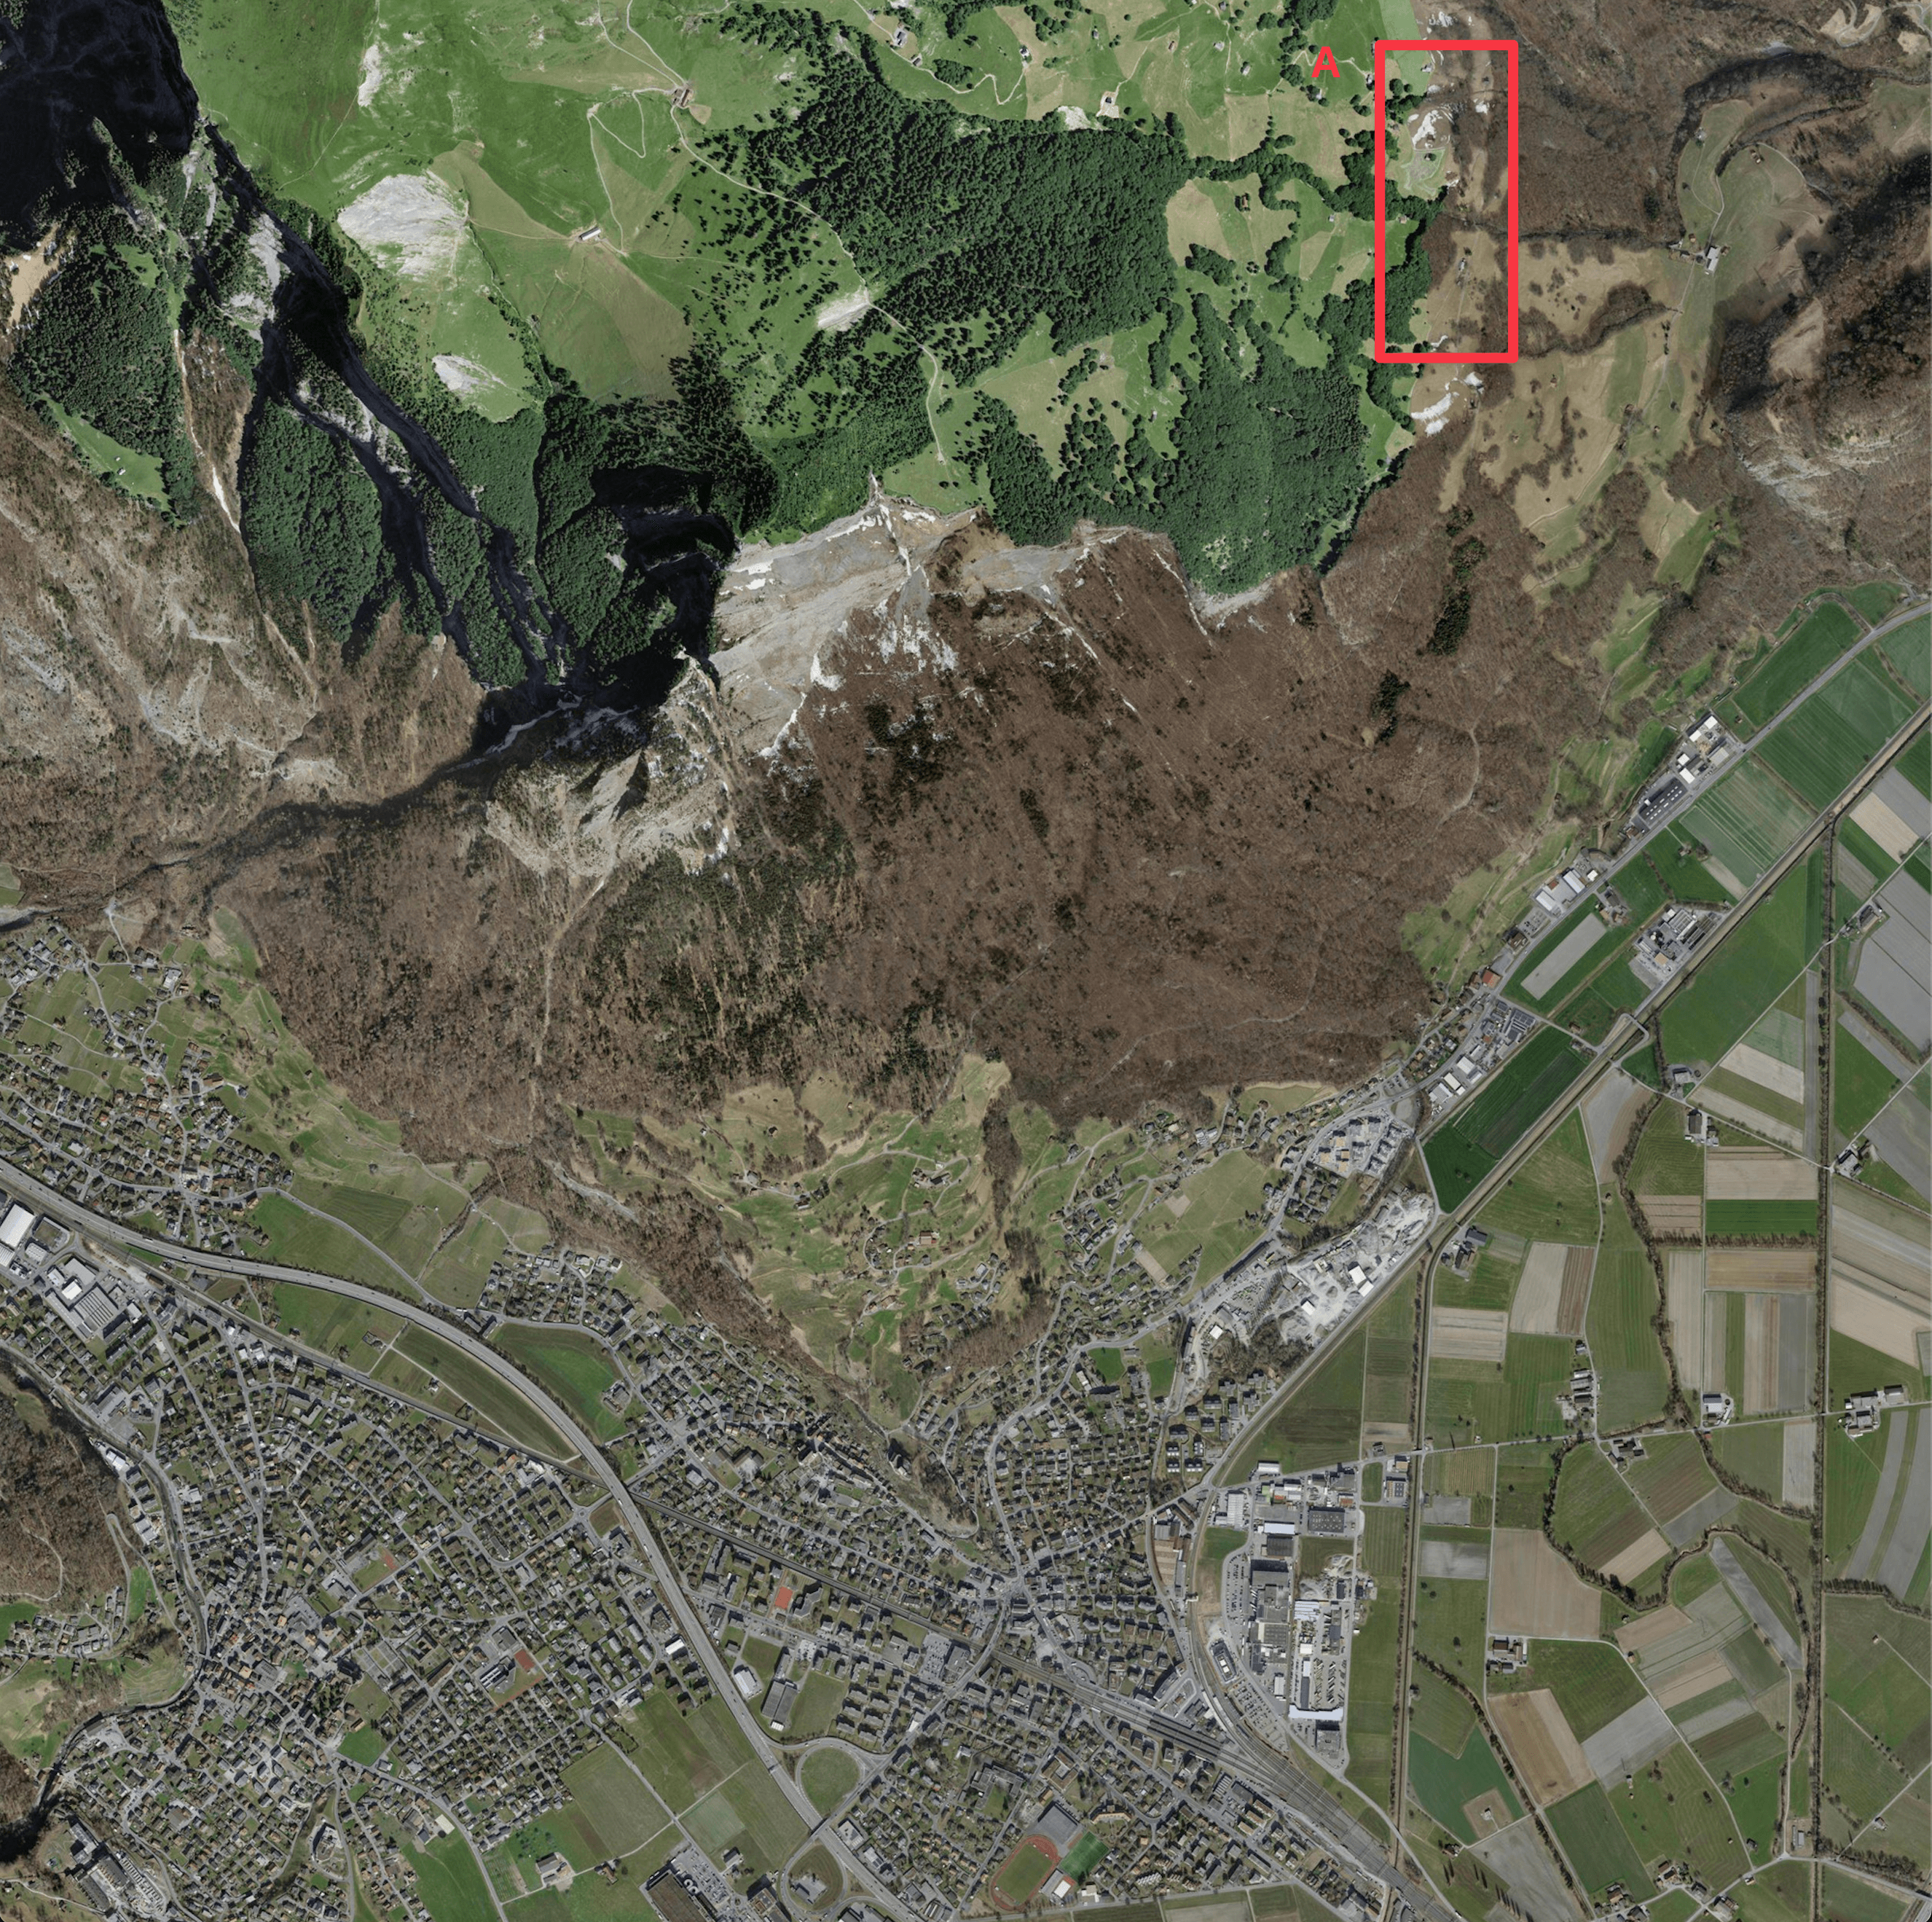
\includegraphics[width=.4\linewidth]{content/00_assets/textur_sargans.png}
    \label{fig_textur_sargans}
\end{figure}

\subsection{Aufteilung in Teilbilder}
Wie bereits in Kapitel \ref{chap_datengrundlage} angesprochen benötigen die Datensätze sowohl von swissALTI3D als auch swissIMAGE, abhängig von der gewählten Auflösung und Detaillierung, entsprechend viel Speicherplatz. Werden die einzelnen km$^2$ Kacheln für den Raum Sargans in der höchsten Auflösung von 10cm pro Bildpixel zu einem Gesamtbild zusammengesetzt, so werden rund 7.5GB Festplattenspeicher benötigt. Obwohl das für native Applikationen, sofern eine genügend schnelle Festplatte vorhanden ist, noch verkraftbar wäre, ist dies beispielsweise im Rahmen einer browserbasierten Anwendung nicht mehr tragbar. Browserbasierte Anwendungen haben gegenüber nativen Applikationen den Vorteil, dass sie von überall aus, ohne Installation, zugreifbar sind. Jedoch müssen die hierfür notwendigen Daten auch auf das Zielsystem des Nutzers heruntergeladen werden. Die Zeit hierfür hängt von der jeweiligen Internetbandbreite ab. Das Herunterladen von grossen Dateien ist daher meistens, trotz Konzepten wie Ladeanimationen etc., keine gute Idee. Um mit grossen Datenmengen auch im Rahmen von webbasierten Anwendungen umzugehen, gibt es andere Methoden.

Um das Problem mit den grossen Bildern zu lösen, wurden zwei Konzepte eingesetzt. Zum einen wurde das Gesamtbild in Teilbider (Tiles) unterteilt, zum anderen wurden diese mit einem bilinearen Downsampling auf eine maximale Auflösung limitiert. Die Teilbilder wurden hierbei, inspiriert von der Quadtree-Datenstruktur, erstellt. Genauso wie es bei einem Quadtree eine entsprechende Baumtiefe gibt, so gibt es bei den Teilbildern ebenfalls unterschiedliche Detaillierungsstufen. Für die erste Stufe (LOD 1) ist das wurde das Gesamtbild in 4 (4$^1$) gleich grosse Teile geschnitten. Für die zweite Stufe sind es hingegen 16 Teilbilder (4$^2$) und so weiter. Abbildung \ref{fig_textur_teilbilder_quadtree} zeigt, wie ein Gesamtbild in Teilbilder mit unterschiedlichen Detailstufen (LODs) aufgeteilt wird. Hierbei sei angemerkt, dass aus Platzgründen nicht alle Teilbilder der Detailstufe LOD2 dargestellt wurden.
\begin{figure}[H]
    \caption{Aufteilung in Teilbilder, angelehnt an die Quadtree Datenstruktur (Eigene Darstellung)}
    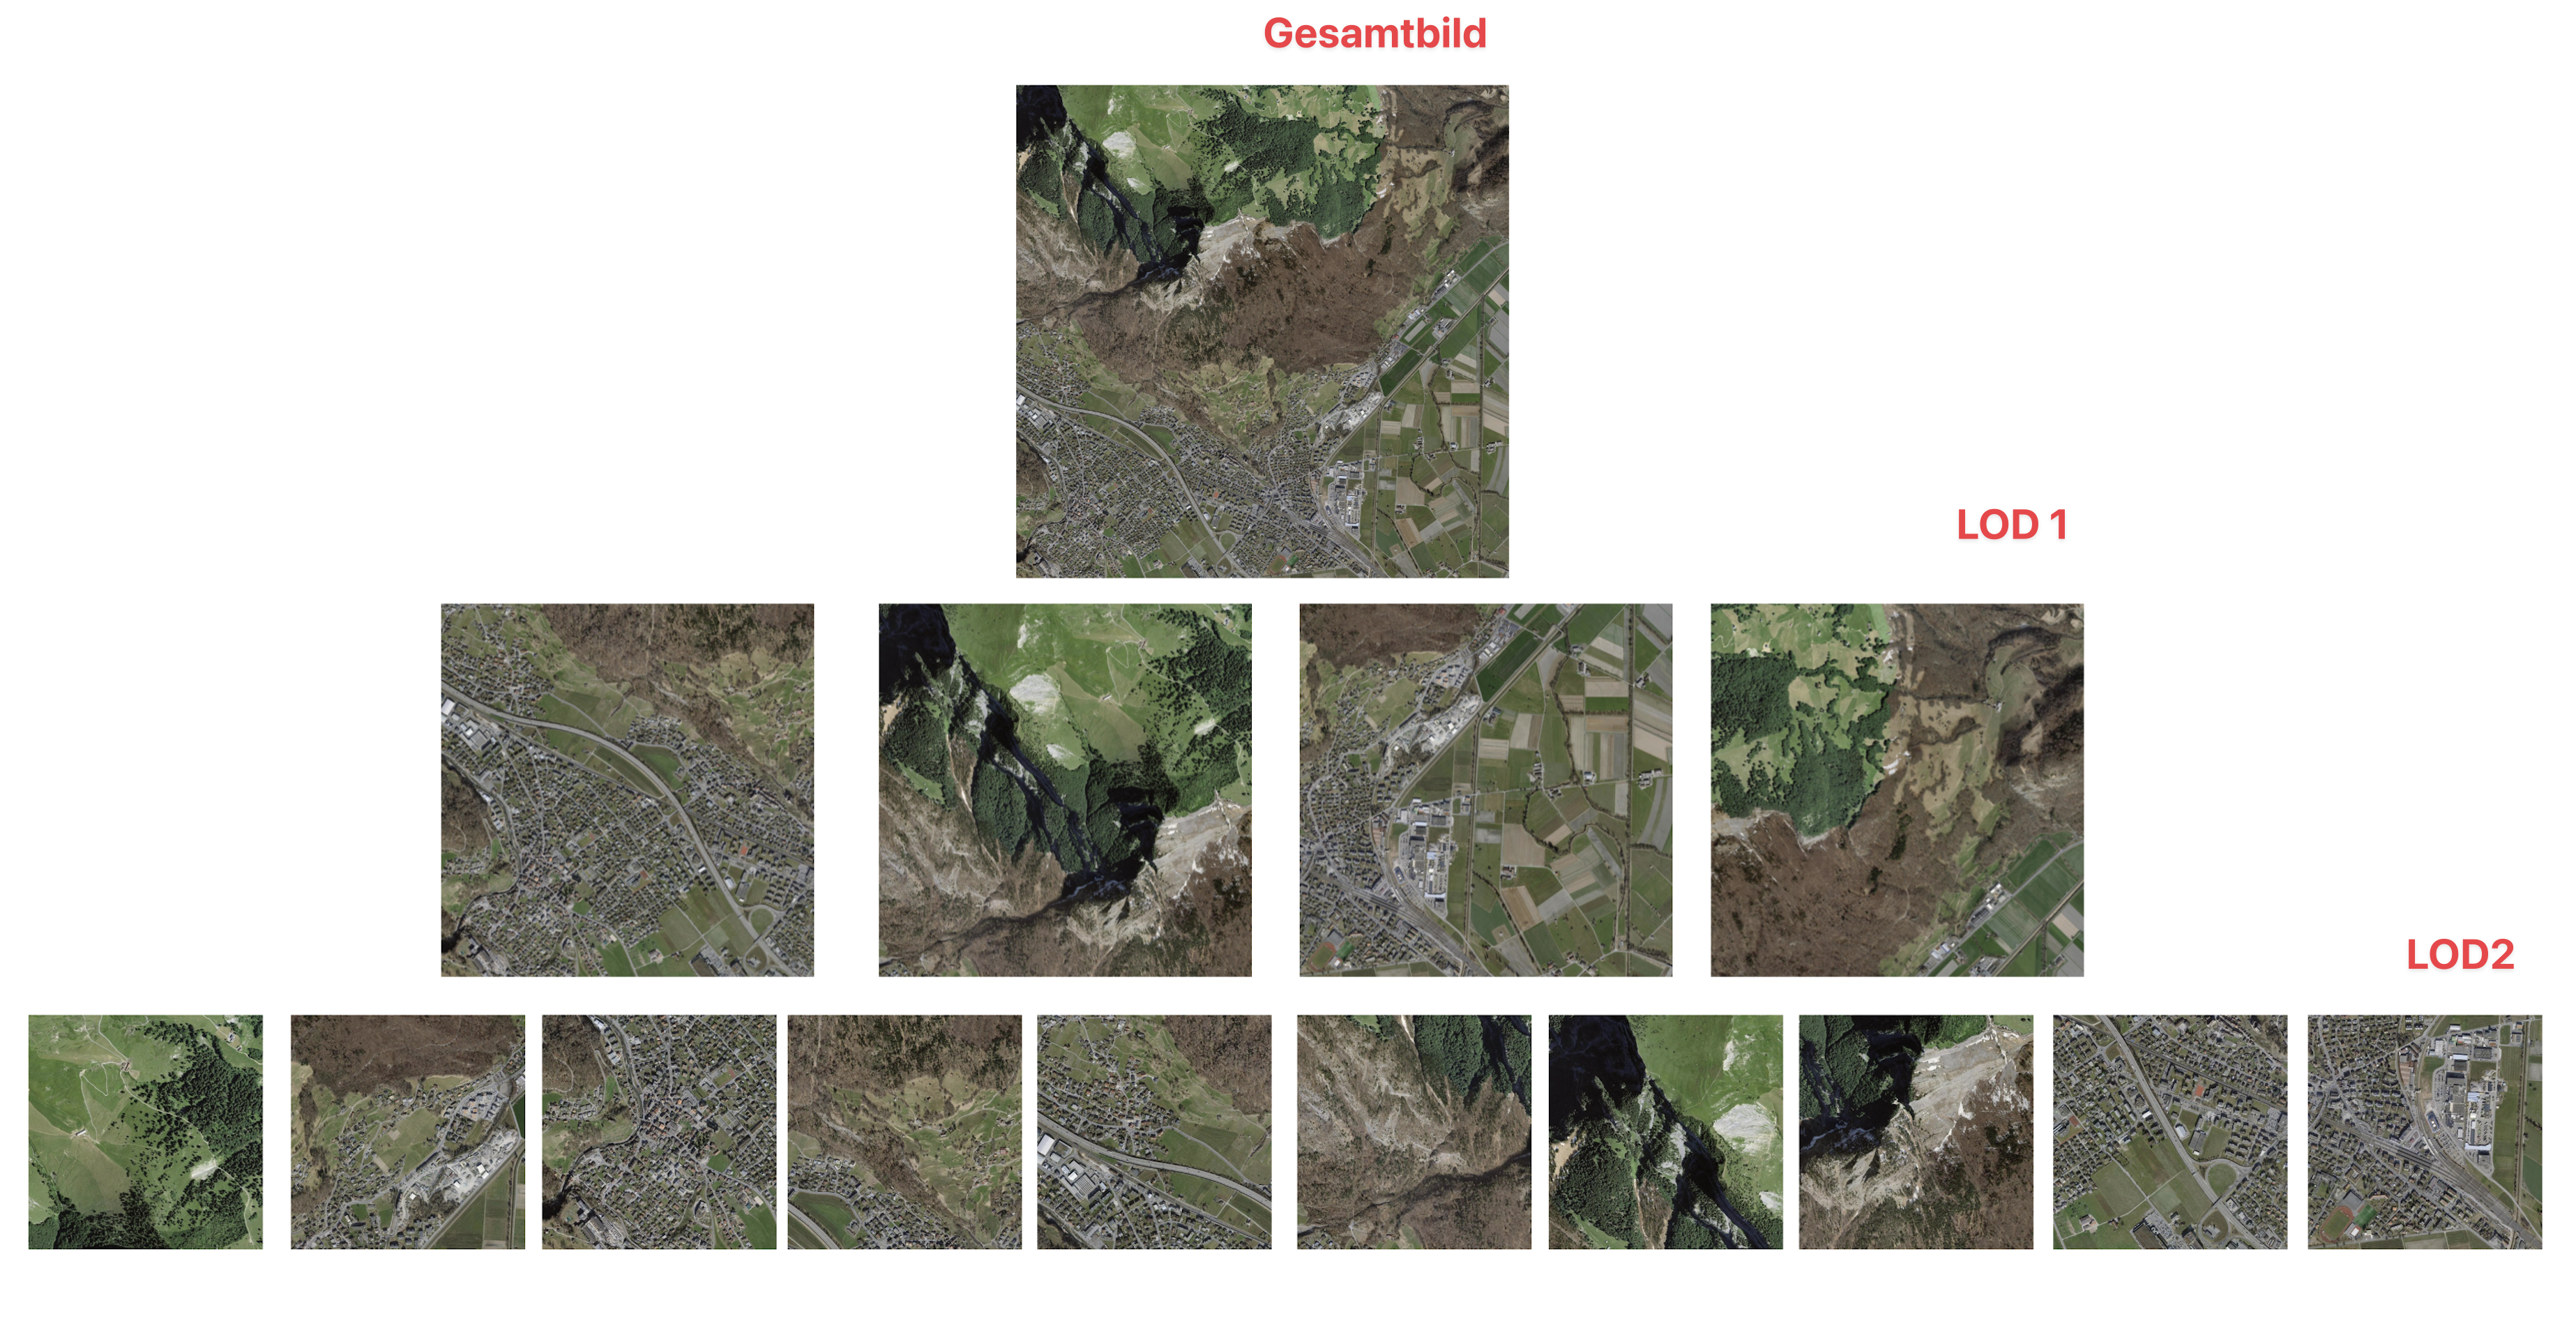
\includegraphics[width=1.0\linewidth]{content/00_assets/zerlegung_in_teilbilder.png}
    \label{fig_textur_teilbilder_quadtree}
\end{figure}

Grafikkarten bevorzugen aus Performanzgründen Texturen mit einer quadratischen Auflösung (500x500 etc.). Jedoch erstrecken sich die swisstopo-Daten je nach Region, nicht immer über einen quadratischen Bereich. Hierzu wird das zusammengesetzte Gesamtbild entsprechend auf einen quadratischen Bildausschnitt begrenzt (siehe Abbildung \ref{fig_begrenzung_bildausschnitt}). 
\begin{figure}[H]
    \caption{Begrenzung Bildausschnitt (Eigene Darstellung)}
    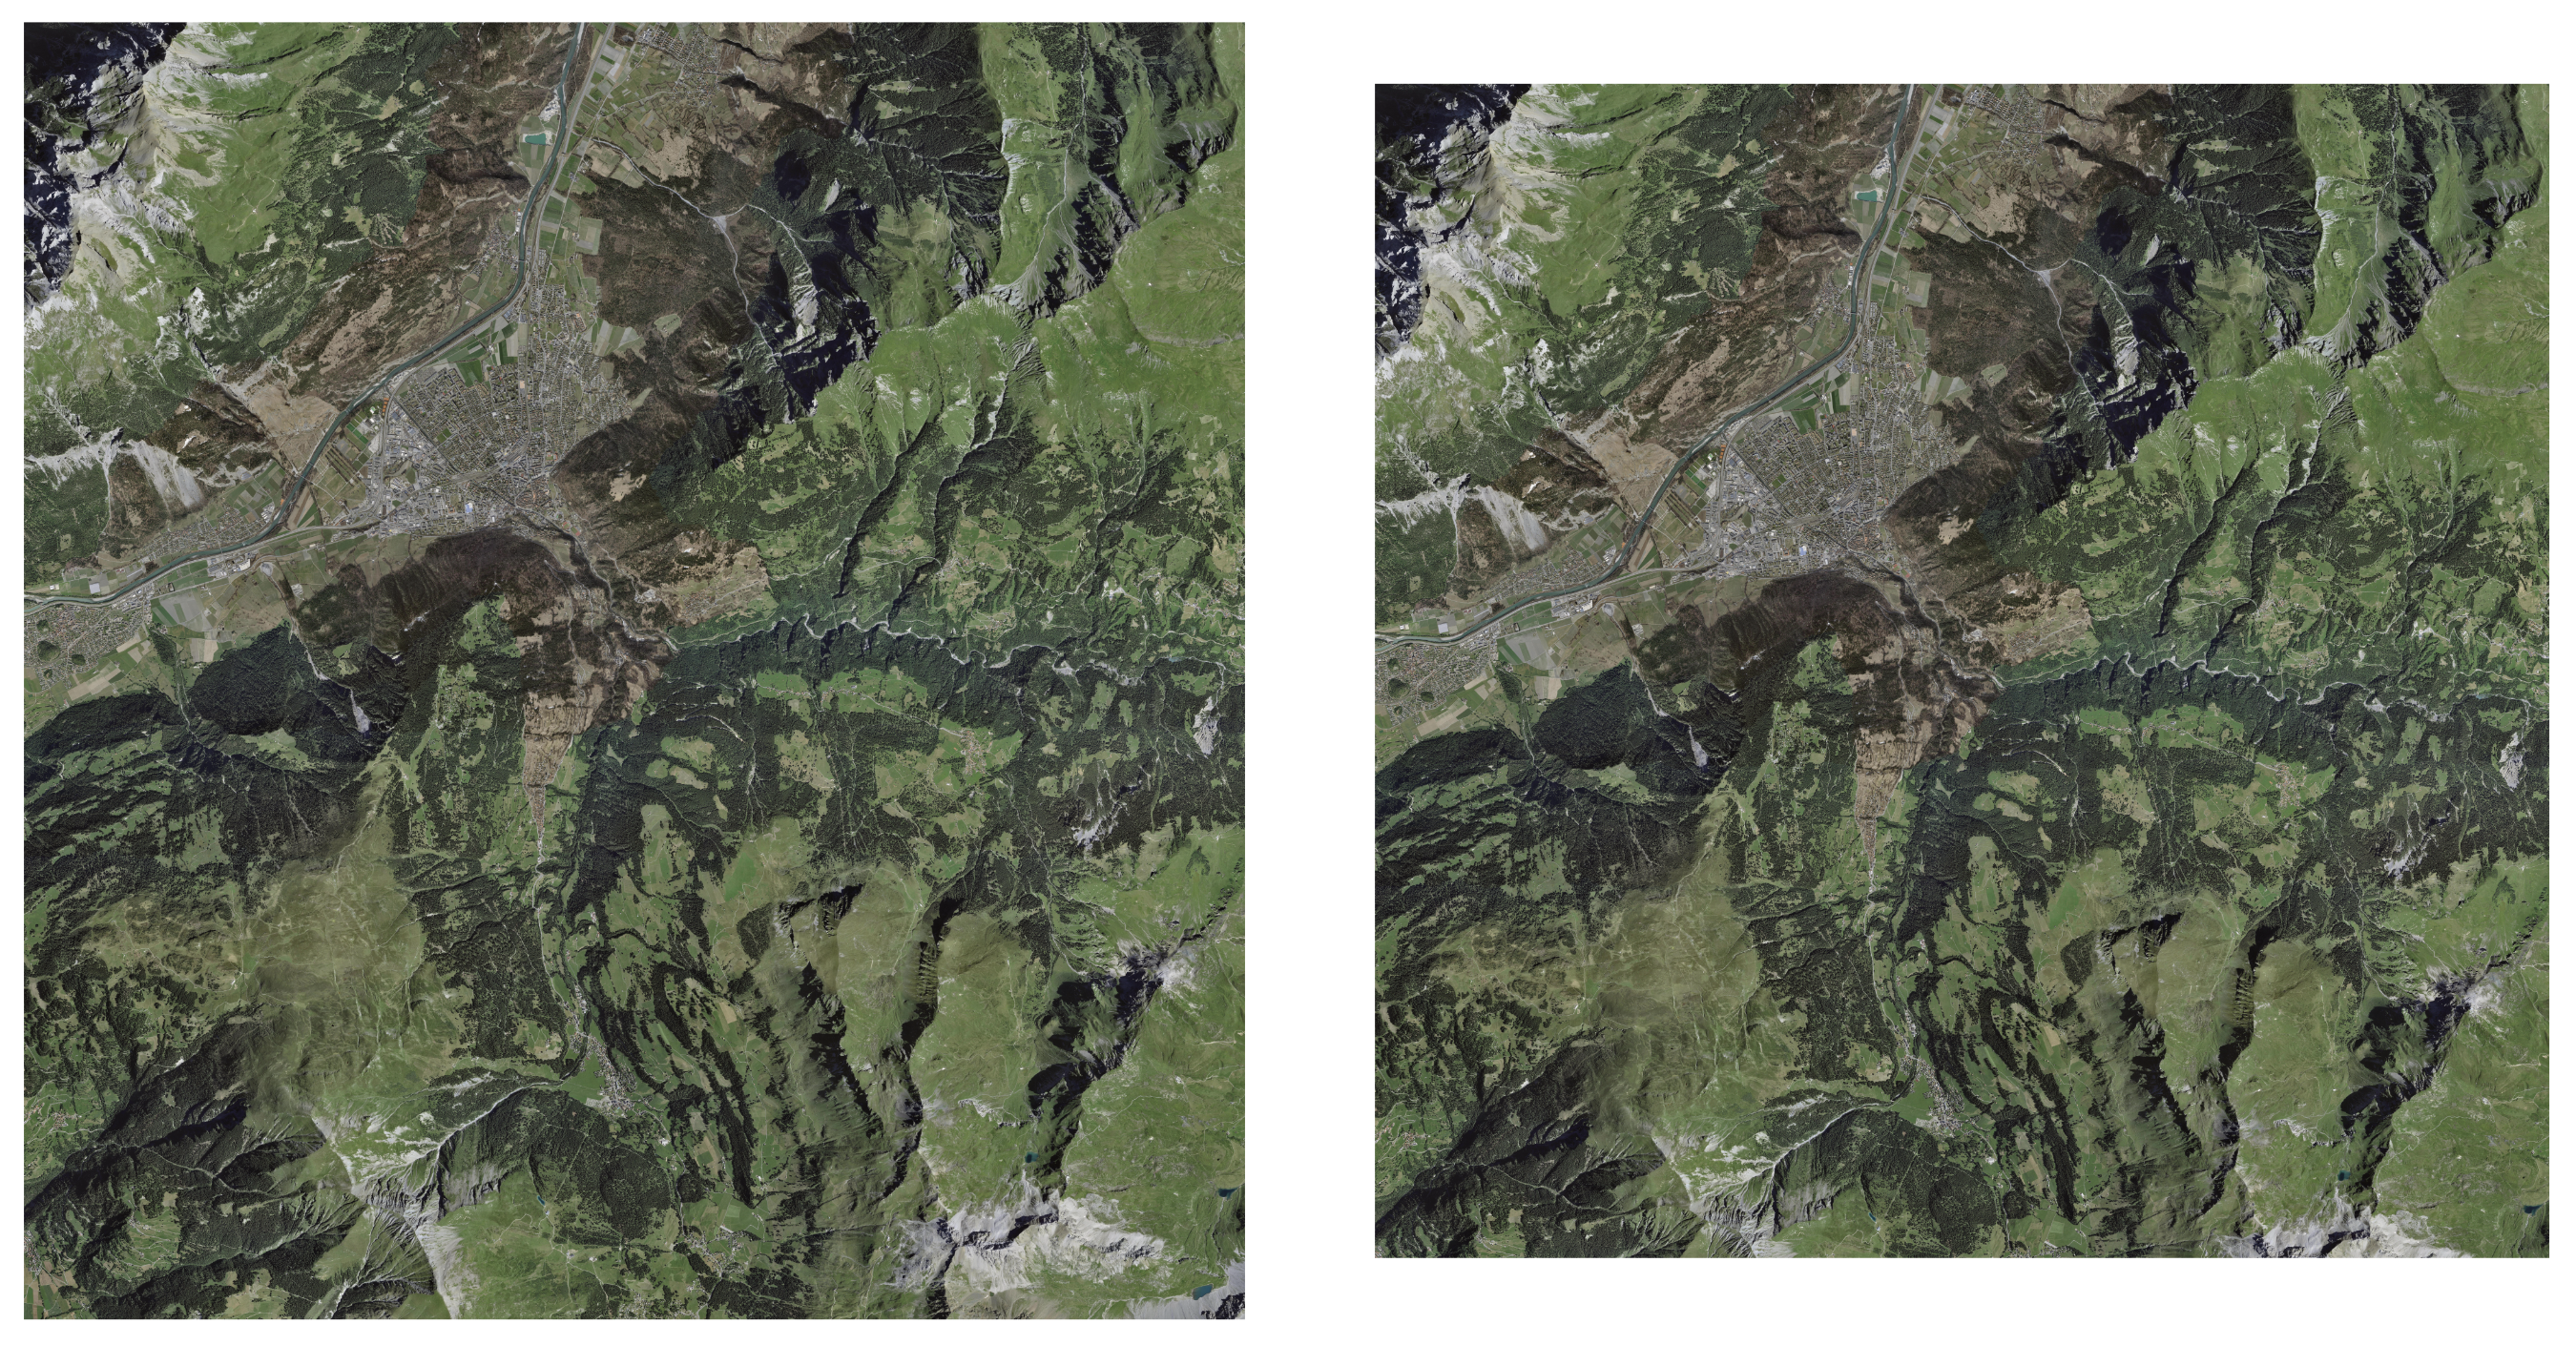
\includegraphics[width=.7\linewidth]{content/00_assets/begrenzung_bildausschnitt.png}
    \label{fig_begrenzung_bildausschnitt}
\end{figure}

\subsection{Automatische Ermittlung der maximalen Baumtiefe}
Die quadratische Begrenzung alleine reicht jedoch nicht aus. Da die Teilbilder anhand der Quadtree-Datenstruktur generiert werden, muss sichergestellt werden, dass in der höchsten Detailstufe (bspw. LOD2 in Abbildung \ref{fig_textur_teilbilder_quadtree}) das Gesamtbild restlos durch die Auflösung einer einzelnen km$^2$ Kachel teilbar ist. Hierfür wird die Logarithmusfunktion verwendet und anhand dieser automatisch die höchste Detailstufe ($L_{\max}$) und infolgedessen die Baumtiefe festgelegt. Hierzu ein Beispiel. Angenommen, das zusammengesetzte Luftbild von Sargans hat eine Auflösung ($R$) von 2000px auf 2000px. Wenn wir davon ausgehen, dass eine km$^2$ Kachel eine Auflösung von 2m pro Bildpunkt hat, ergibt sich somit eine Auflösung ($T$) von 500px ($\frac{1000m}{\frac{2m}{1px}}$) pro km$^2$. Mithilfe der unten stehenden Formel ergibt sich hiermit eine maximale Baumtiefe von 3.

\[
L_{\max} = (\log_2\frac{R}{T}) + 1
\]

\subsection{Border Patching}
Mithilfe der extrahierten Höhen sowie Bildinformationen ist es nun möglich, 3D-Modelle zu rekonstruieren. Auf die genaue Generierung der 3D-Modelle wird in Kapitel \ref{chap_erstellung_geometrie} eingegangen. Werden die 3D-Modelle aneinandergereiht, so wird jedoch ersichtlich, dass sich Risse an den angrenzenden Randbereichen bilden (siehe schwarze Bereiche in Abbildung \ref{fig_risse_zwischen_3d_modellen}). Grund hierfür ist folgender. Das Gesamtbild wird, wie bereits erwähnt, in Teilbilder zerschnitten. Die Höhendaten weisen jedoch an den entsprechenden Schnittkanten nicht die gleichen Werte wie ihre angrenzenden Nachbarn auf. Dementsprechend divergieren die Position der Vertices und es entstehen Risse.
\begin{figure}[H]
    \caption{Risse zwischen 3D Modellen der gleichen Detailstufe (Eigene Darstellung)}
    \includegraphics[width=.5\linewidth]{content/00_assets/risse_zwischen_gleichen_detailstufen.png}
    \label{fig_risse_zwischen_3d_modellen}
\end{figure}

Diese Problematik kann jedoch mithilfe von Broder Patching eliminiert werden. Die Idee hierbe ist, dass an den entsprechenden Rändern der Bilder jeweils Daten der angrenzenden Nachbarn übernommen werden und so ein Überlappungsbereich geschaffen wird. Ein Überlappungsbereich von bereits einem Pixel genügt, um die Risse komplett zu eliminieren.

\subsection{Relative Geopositionsinformationen}
ThreeJs hat wie die swisstopo-Daten einen Koordinatenursprung. Dieser Mittelpunkt befindet sich jedoch nicht wie bei swisstopo an den Koordinaten (2'600'000/1'200'000), sondern an der Stelle (0/0). Damit die 3D-Visualisierung um den ThreeJs Mittelpunkt positioniert werden kann, werden daher relative Geopositionsinformationen berechnet. Hierzu wird in einem ersten Schritt der Mittelpunkt des zusammengesetzten Gesamtbildes berechnet. Anschliessend wird bei der Erstellung der einzelnen Teilbilder der relative Abstand zu diesem Mittelpunkt bestimmt. Hiermit ist sichergestellt, dass die 3D-Modelle relativ um den ThreeJs Koordinatenursprung platziert werden können.

\subsection{Generierung von Metadaten}
Um wichtige Informationen zu den generierten Daten nicht zu verlieren, werden entsprechende Metadaten generiert. Diese werden in Form einer JSON-Datei abgespeichert und können somit zur Laufzeit der Webanwendung eingelesen werden. Abbildung \ref{fig_ausschnitt_metadaten} zeigt einen Ausschnitt aus den automatisch erstellten Metadaten. In den Metadaten stehen relevante Informationen wie:
\begin{itemize}
    \item Absolute Geopositionsinformationen im LV95-Koordinatensystem
    \item Relative Geopositionsinformationen im LV95-Koordinatensystem
    \item Maximale Baumtiefe (LOD)
    \item Globale Maximum und Minimum der Höheninformationen
    \item Dateipfade zu den generierten Bilddateien
\end{itemize}

\begin{figure}[H]
    \caption{Auszug aus den generierten Metadaten (Eigene Darstellung)}
    \includegraphics[width=.8\linewidth]{content/00_assets/ausschnitt_metadaten.png}
    \label{fig_ausschnitt_metadaten}
\end{figure}

\newpage

\section{Implementierung}
TODO

\subsection{Erstellung der Geometrie}
\label{chap_erstellung_geometrie}
TODO

\subsection{Algorithmen}
TODO

\subsection{Hilfsvisualisierungen}
TODO

\section{Performance Messung}
TODO

\section{Optimierungen}
TODO